\section{Test Environment}

The test environment mainly serves two purposes. First, it makes it easy to evaluate and compare the performance of different probabilistic model learning techniques, according to the Pautomac evaluation criteria described in \todo{Insert secref}.
Second, it makes it more convenient to experiment with the creation of new techniques by allowing reuse or altering of different techniques or parts thereof, that has already been implemented. In \ref{fig:testenvironment} an overview of the test environment is given.

\begin{figure}[!htb]
\centering
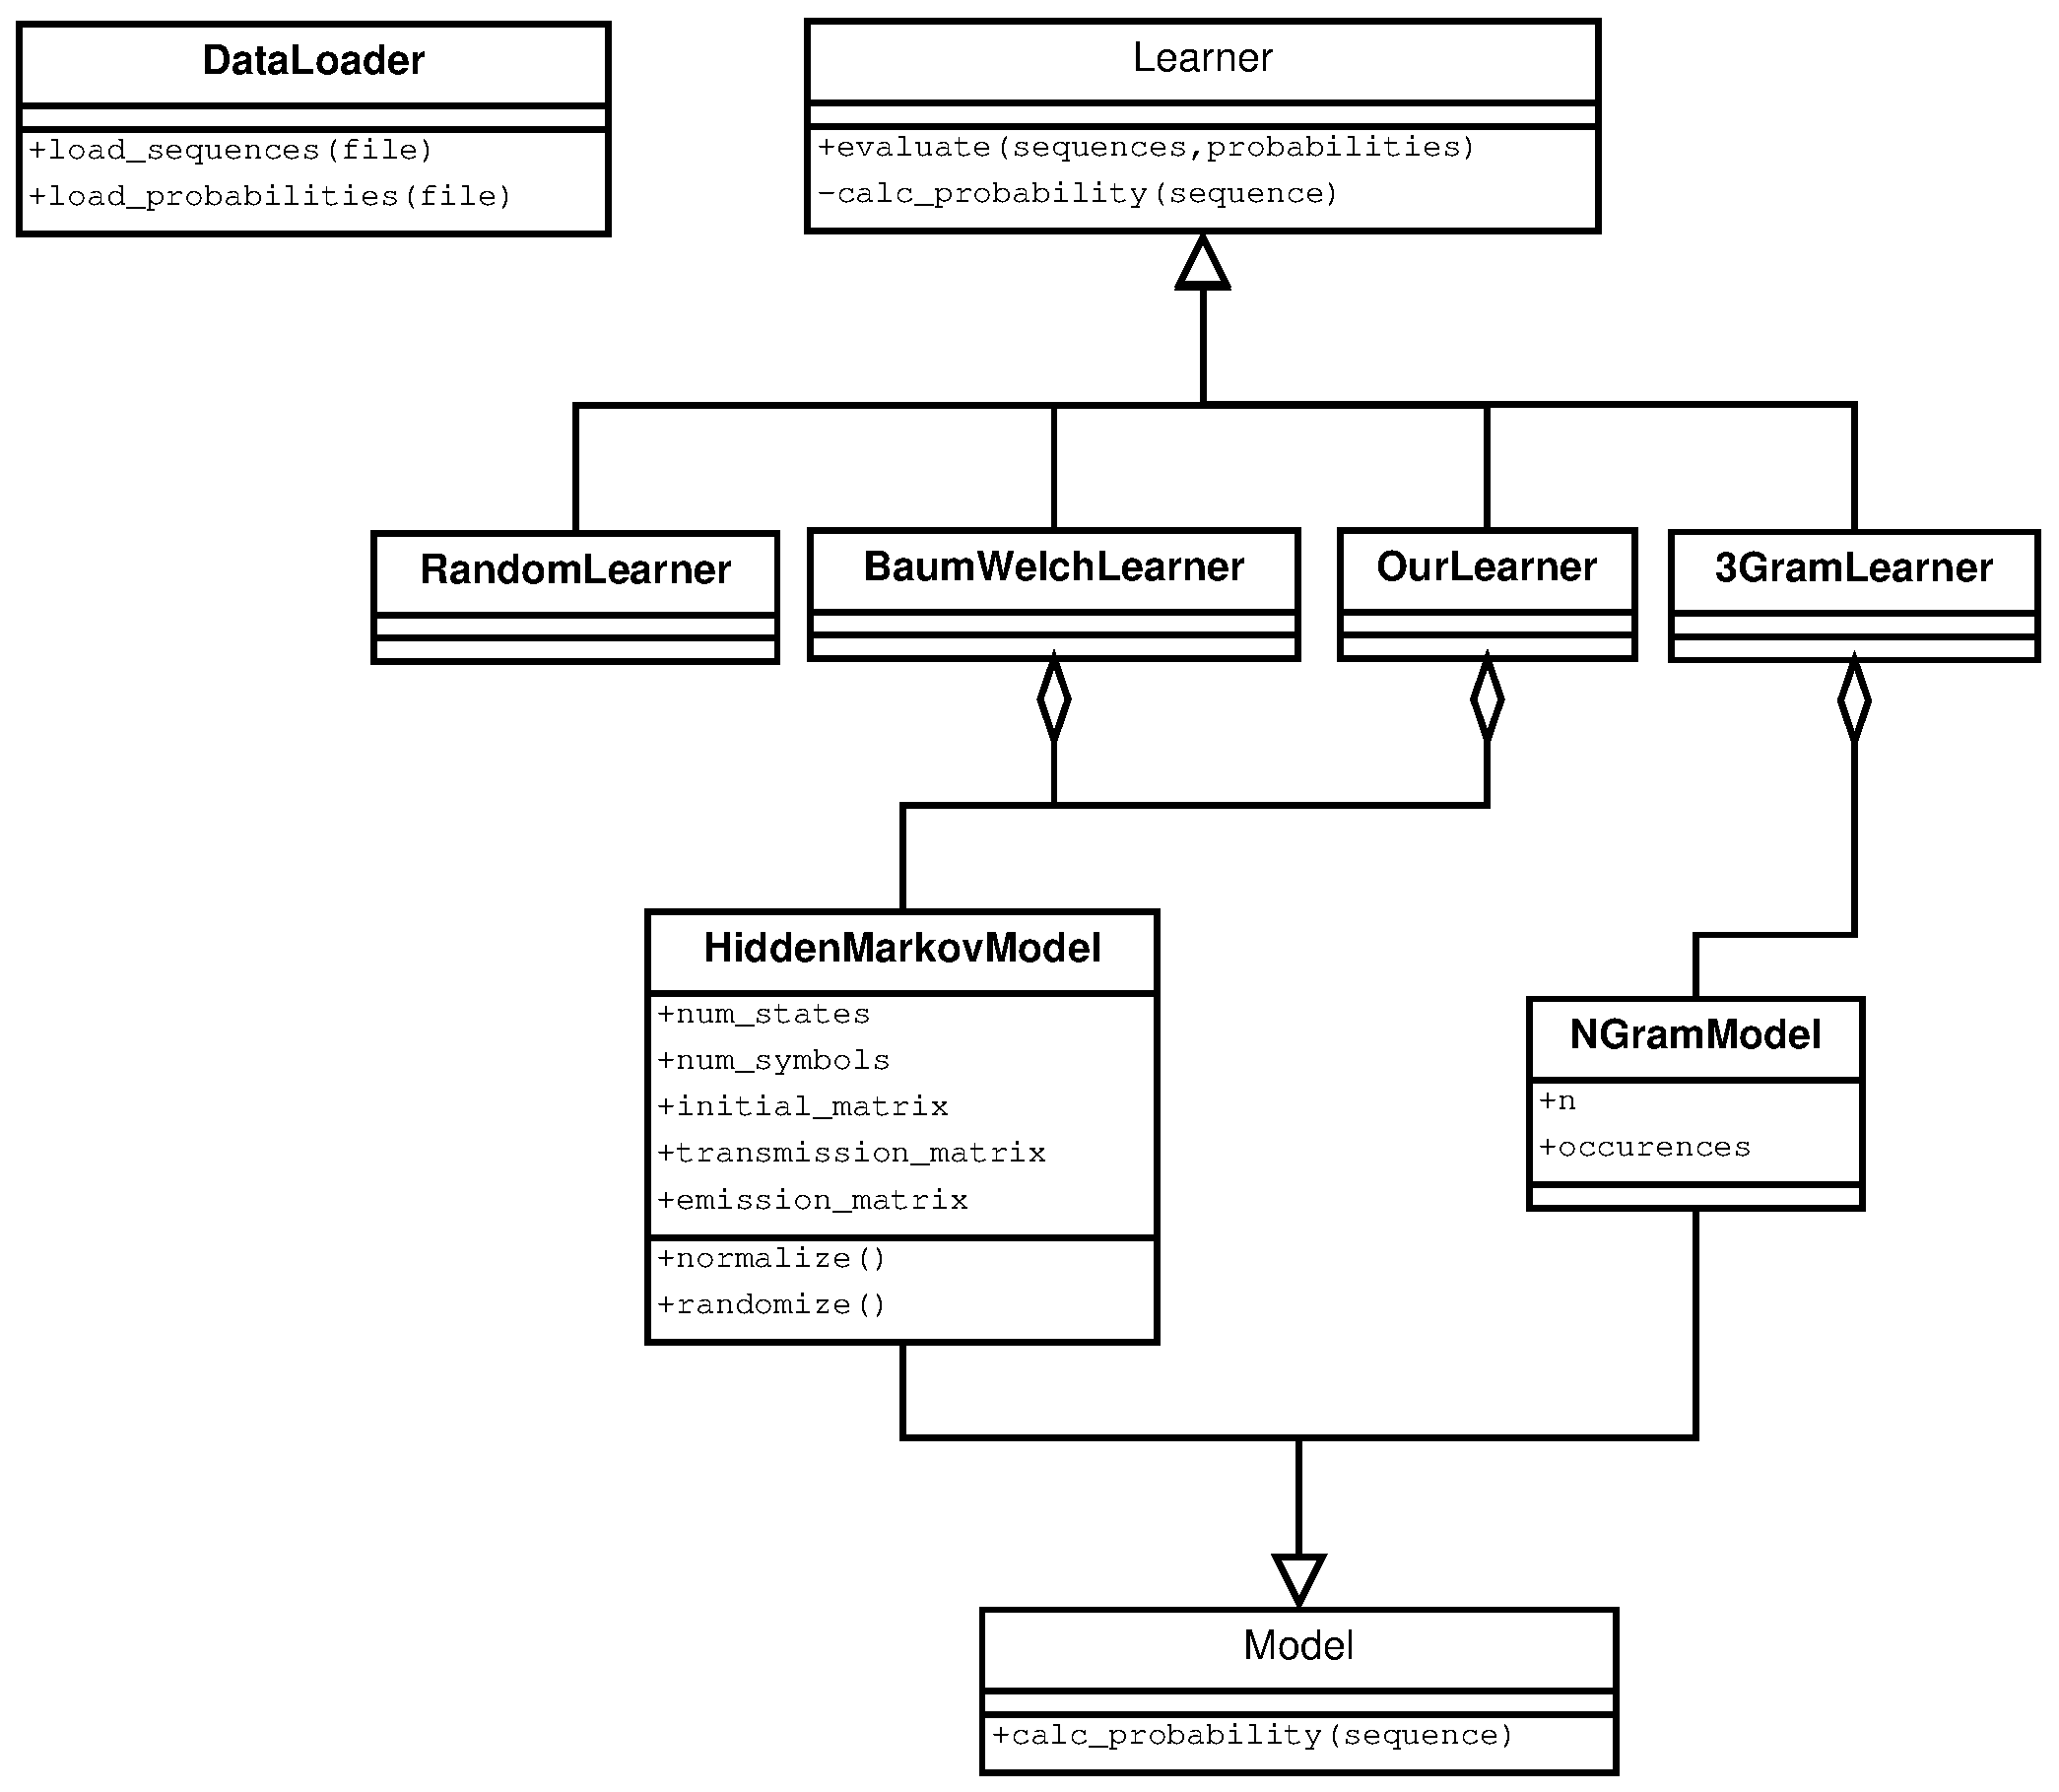
\includegraphics[scale=.4]{pictures/test-environment-overview.eps}
\caption{An overview of the test environment}
\label{fig:testenvironment}
\end{figure}

\subsection{DataLoader}
The \formatclass{DataLoader} class is responsible for loading both training data, test data and solution data from the files published at the Pautomac website. Both training and test data is represented by a list of sequences, while solution data is represented by a list of probabilities.
This class contains the two functions \formatfunction{load\_probabilities\_from\_file(file\_path)} and \formatfunction{load\_sequences\_from\_file(file\_path)}. The file to be read by both functions must be formatted according to the Pautomac data formats, as described in \todo{insert secref}. The former function outputs a list of sequences, where each sequence is represented by a list of integers.
The latter function outputs a list of probabilities, where each probability is represented by a floating point.

\subsection{Learner}
If one wants to implement a new technique for learning the parameters of a probabilistic model, a new class must be created that derives from the abstract class \formatclass{Learner}.
A learner has only one responsibility: Given a list of training sequences, it must learn a probabilistic model as close as possible to the model used to generate those sequences. How this is done is up to the implementer to choose. The only requirement is that he implements a \formatfunction{calc\_probability(sequence)} function, which given a sequence should return how likely it is that the learned model generated that sequence.
The \formatclass{Learner} class has an already implemented function called \formatfunction{evaluate(sequences, probabilities)}, which uses the \formatfunction{calc\_probability(sequence)} function to calculate probabilities for all provided sequences.
The probabilities are then normalised, and a score is calculated based on the Pautomac evaluation criteria.
The \formatfunction{evaluate} function can be seen by \ref{code:learner}.
A learner should also define a name.

\subsection{Model}
Consider one \formatclass{Learner} that uses the Baum Welch algorithm to estimate the parameters of a Hidden Markov Model and a second \formatclass{Learner} that uses another algorithm, also for estimating the parameters of a Hidden Markov Model. The two learners may need to do many of the same operations on a Hidden Markov Model, e.g. normalization, calculating the probability of being in a particular state or observing a particular sequence at a given time. 
It would be time consuming and increase redundancy if both learners were to implement their own Hidden Markov Model and operations on it.
The \formatclass{Model} has been created to facilitate this. It is an abstract class, which only dictates that a single function must be implemented, which is the \formatfunction{calc\_sequence\_probability(symbol\_sequence)} function. Given a sequence, it must return the probability for the model to generate that sequence. Note that this function is intended to be directly used as the output of the function in the \formatclass{Learner} class having the same name.

\begin{figure}
\caption{The \formatfunction{evaluate} function of the \formatclass{Learner} class.}
\label{code:learner}
\pythonexternal{codeexamples/learner.py}
\end{figure}


\subsection{Evaluator}
This class is responsible for evaluating a \formatclass{Learner} according to the Pautomac evaluation criteria.
Given a learner that has already learned a model, and a number of test sequences with their respective probabilities, it checks how well the probabilities predicted by the \formatclass{Learner} matches the real probabilities.


\subsection{Benchmarker}
For evaluating particular learners on particular data sets, the \formatclass{Benchmarker} class is convenient to use.
As input, it takes a set of learners and data sets, a number of runs, and an output file path.
When run, the \formatclass{Benchmarker} will load all the data sets using the \formatclass{DataLoader}. A data set contains training sequences, test sequences, and a probability associated with each test sequence. For each run, the \formatclass{Benchmarker} randomly splits the training sequences into two sets, where the first $\frac{2}{3}$ sequences are used for training while the remaining are used for validation during training.
Each \formatclass{Learner} will attempt to learn an underlying model for each of the data sets, one by one. When having learned a model for a particular data set, it is evaluated by the \formatclass{Evaluator}. The result of the benchmark is a mean and median score for each pair of learner and data set, which is output to a specified file in .csv format. Besides the mean and median score, the mean and median running time is also measured.